\section{Arquitetura de solução}

A arquitetura da solução é baseada, de uma forma geral, na arquitetura \ac{mvc}. Este modelo é apresentado em camadas que separam a apresentação e a interação de dados no sistema. É estruturado em três componentes: o modelo, que é o responsável pelo gerenciamento dos dados, a visão, que gerencia a apresentação dos dados, e o controlador, responsável por intermediar a comunicação entre os eventos gerados pelo usuário na interface e o modelo \cite{engenharia-de-software:2018}.

O diagrama apresentado pela \autoref{fig:arquitetura}, mostra o modelo arquitetural.

\begin{figure}[htb]
    \centering
	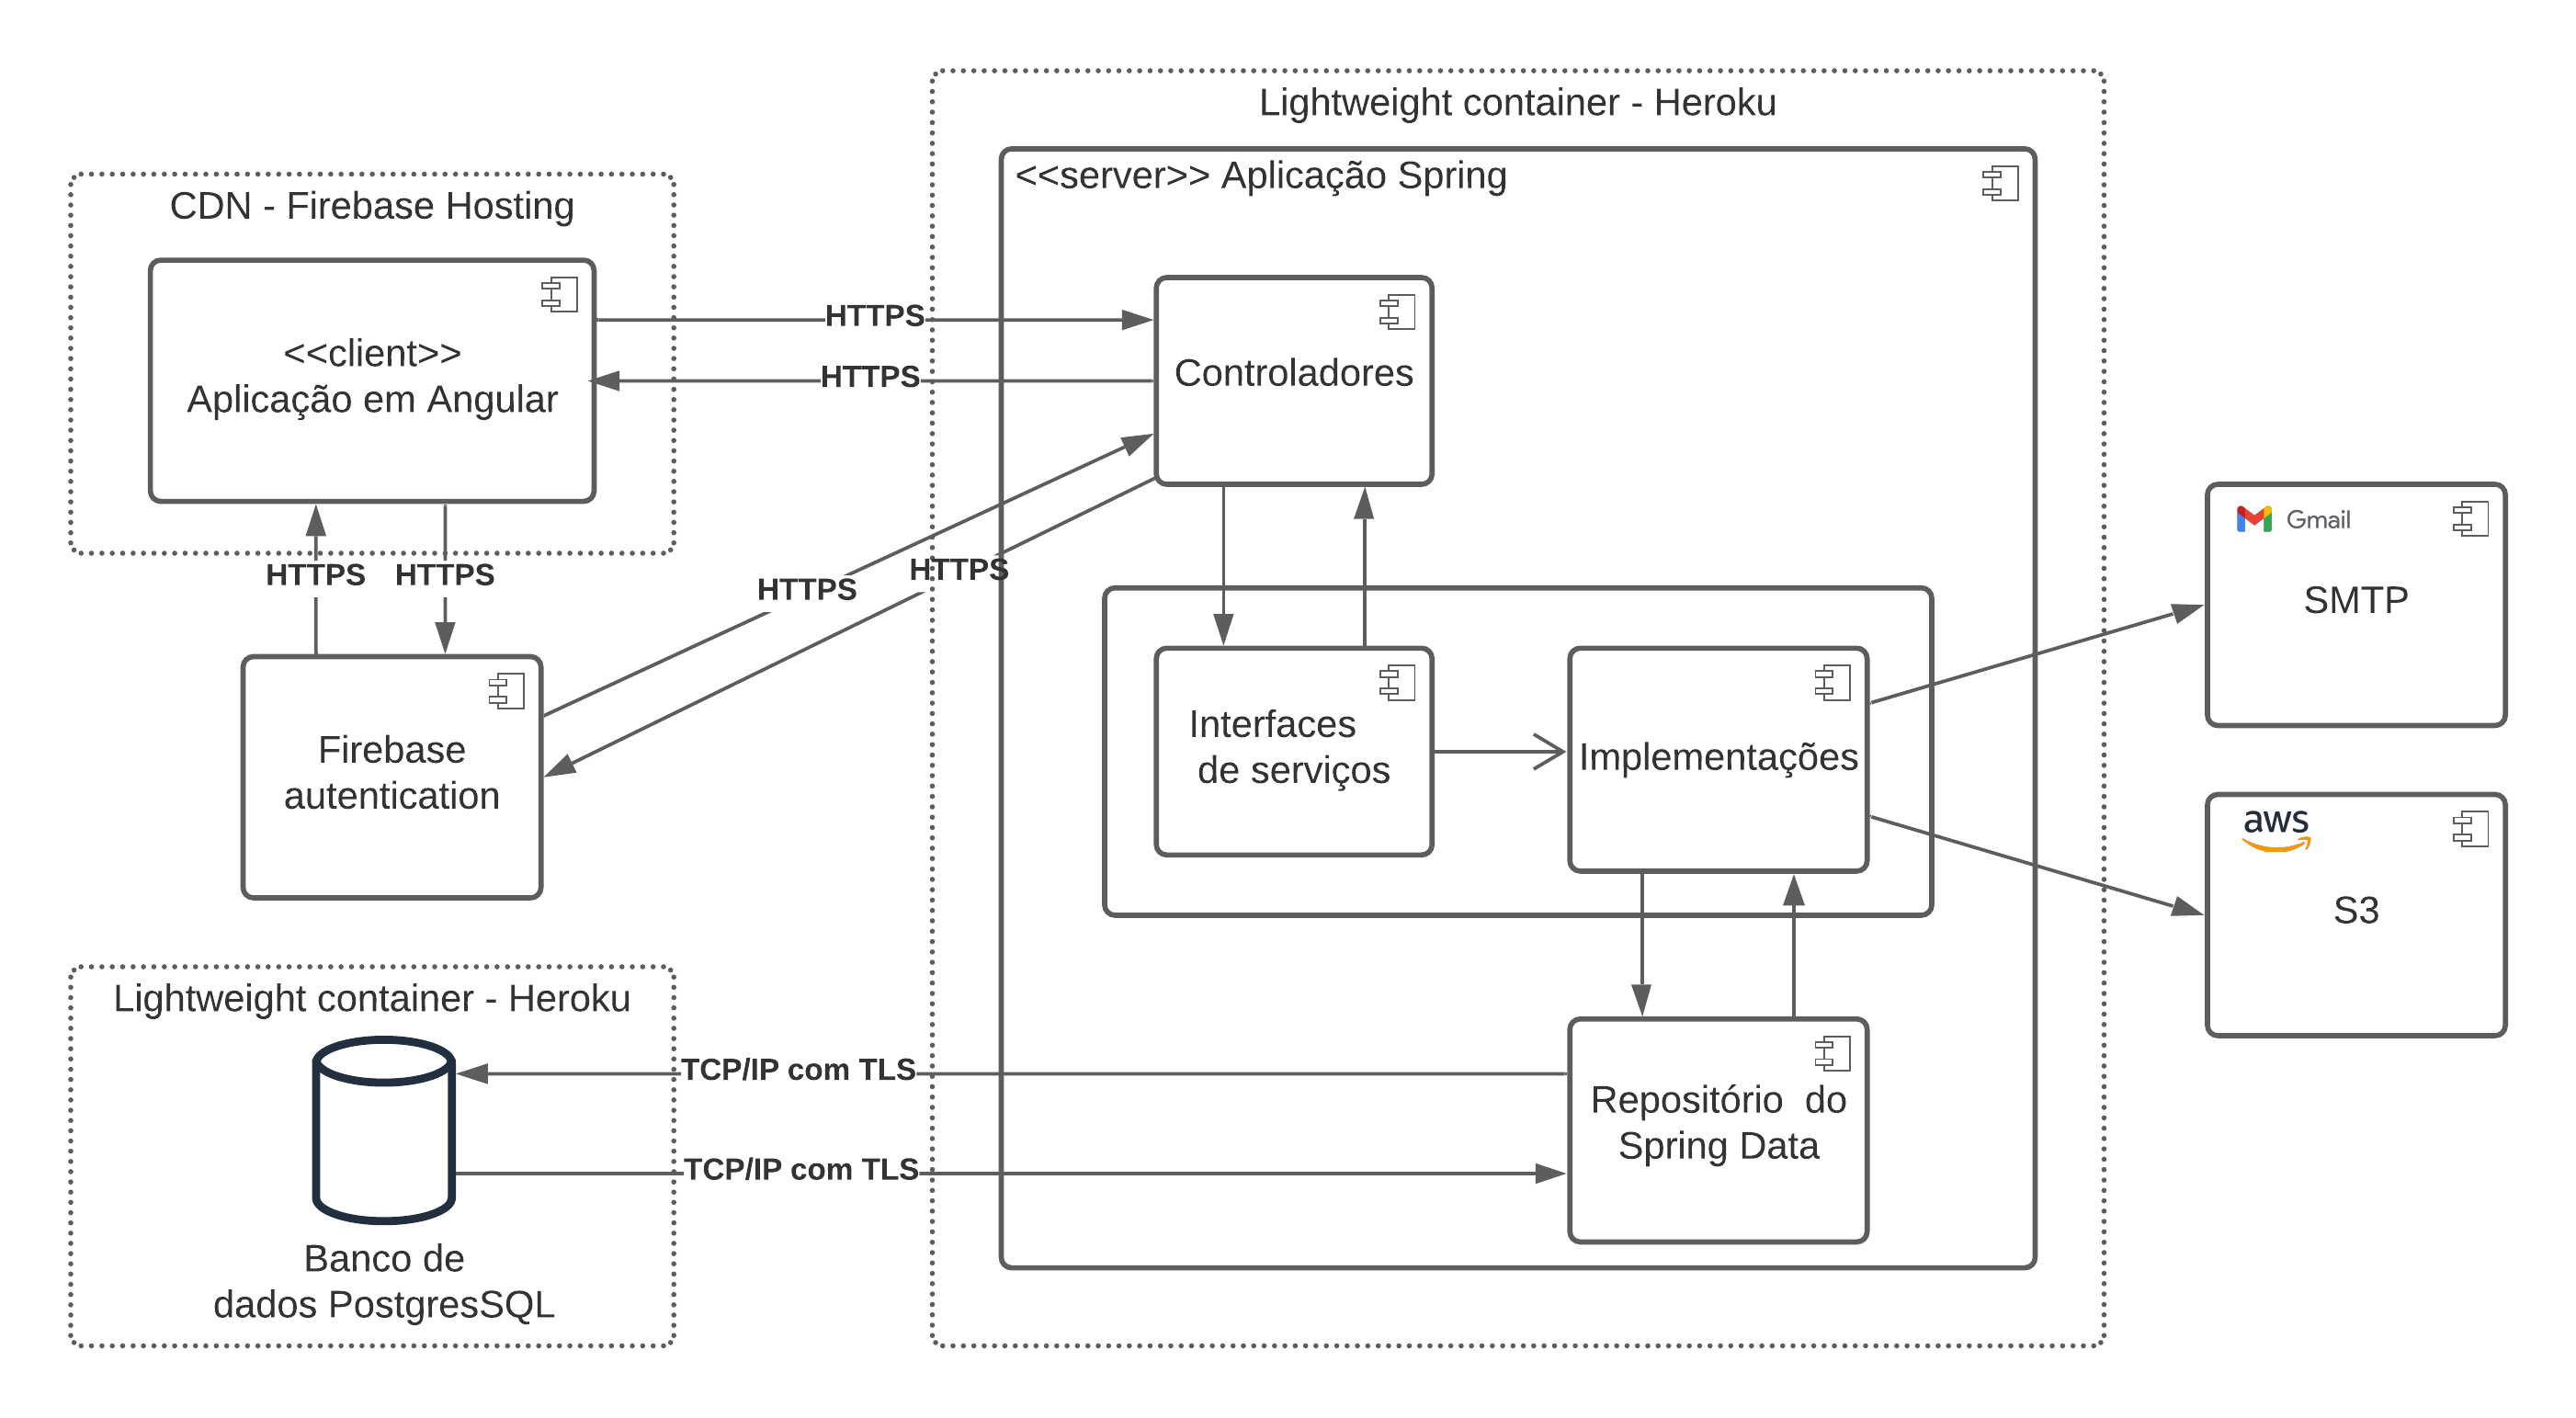
\includegraphics[width=16cm]{imagens/Arquitetura.png}
	\caption{\label{fig:arquitetura} Arquitetura da solução}
	\fonte{Os autores}
\end{figure}
 
 
De modo a desenvolver uma aplicação que busca garantir uma boa usabilidade e capaz de aproveitar os recursos disponíveis da melhor forma, para a interface do usuário (\textit{\gls{front-end}}) será adotado o modelo arquitetural \ac{spa}. 


Neste modelo, a maioria dos recursos necessários é carregada na inicialização da aplicação, fazendo com que não seja necessário recarregar a página durante o uso. A única mudança que ocorre é a dos dados, que são trafegados entre o servidor e o cliente.


Conforme o diagrama apresentado pela \autoref{fig:arquitetura}, as camadas que compõem a solução utilizam as seguintes infraestruturas para hospedagem:
\begin{itemize}
\item \ac{cdn} (Firebase Hosting): infraestrutura responsável por hospedar a aplicação em Angular, da camada de visão. Um serviço de hospedagem, que tem como base o armazenamento em \ac{ssd} e uma \ac{cdn}, totalmente gerenciado para conteúdo estático e dinâmico.
\item  Lightweight container (Heroku): infraestrutura responsável por hospedar a aplicação Spring da camada controladora e o banco de dados da camada de modelo. A tecnologia utilizada pelo Heroku, utiliza o conceito de \textit{\gls{container}} que empacota o código e as dependências do aplicativo abstraindo o gerenciamento do \textit{\gls{hardware}}, levando a simplificação do desenvolvimento e o aumento da produtividade.
\end{itemize}

Para a autenticação da aplicação, é utilizado o Firebase Authentication. E para minimizar os impactos negativos da utilização de uma tecnologia terceira, o Firebase Authentication é implantado seguindo o padrão de projeto \textit{Adapter}. Deste modo, diante da necessidade, a tecnologia pode ser facilmente substituída por outra ou até mesmo por uma proprietária.

Para finalizar a composição da arquitetura da aplicação foram adicionadas duas implementações. O \ac{smtp} do Gmail, protocolo responsável por apoiar o envio e-mails da aplicação. E o S3 da Aws, serviço responsável pelo armazenamento dos documentos de atividades.


A comunicação entre a camada de visão e a camada controladora será realizada via protocolo \ac{https}. Este protocolo acrescenta uma camada a mais de segurança à aplicação, uma vez que utiliza a criptografia na transferência de recursos.


Já a comunicação entre os controladores e banco de dados, é realizada via \ac{tcpip} acrescido do protocolo \ac{tls} que aumenta a segurança através de criptografia, a interoperabilidade, a extensibilidade e a eficiência.


